\subsection{Larvas}
Para el análisis de la tasa de desarrollo, en días, de las larvas, del Aedes aegypti, incluyeron
aquellas que culminaron su estado para pasar a ser una pupa. Existen diversos
estudios, que han reportado que tasa de desarrollo de las larvas, se encuentra influenciada por la
temperaturura y varia de acuerdo a las localidades y subespecies. A continuación se mencionaran
algunos estudios realizados correspondientes a la tasa de desarrollo en días de la larva, con el
fin de realizar una comparación con los resultados obtenidos.

En \cite{rueda1990temperature}, se reporta el efecto de  temperaturas constantes sobre las tasas
de desarrollo, el crecimiento y la supervivencia de los estados inmaduros de Aeedes aegypti,
determinadas en condiciones de laboratorio, y el modelo dependiente de la temperatura de
\cite{sharpe1977reaction}. En la \tabref{tab:desarrollo-larva-rueda1990temperature-test} se
presentan los resultados obtenidos a seis temperaturas constantes(15-34 \textcelsius) en
comparación a los obtenidos en \cite{rueda1990temperature}.


\begin{table}[H]
    \begin{minipage}{\textwidth}
        \centering
        \caption{ \label{tab:desarrollo-larva-rueda1990temperature-test} Análisis de la tasa de desarrollo de las larvas del Aedes Aegypti a seis temperaturas constantes
        (15-34 \textcelsius).}
        \begin{tabular}{p{5cm} c c c c c c c}
            \hline\\
            Resultados & 15\textcelsius & 20\textcelsius & 25\textcelsius & 27\textcelsius
            & 30\textcelsius & 34\textcelsius &  Media General\\
            \hline
            \hline \\
            Media Observada$^{a}$   & 46,83 & 9,31  & 8,61 & 4,47 & 4,99 & 5,06 & 13,21\\
            Mediana Observada$^{a}$ & 45,82 & 9,06  & 8,7  & 4,46 & 4,86 & 5,04 & 12,99\\
            Media Predicha$^{b}$    & 42,33 & 14,89 & 6,48 & 5,28 & 4,72 & 5,61 & 13,22\\
            Media obtenida$^{c}$    & 44,34 & 14,99 & 6,62 & 5,53 & 4,47 & 5,6 & 13,59\\

        \end{tabular}
        \footnotetext[1]{Valores observados por \cite{rueda1990temperature}.}
        \footnotetext[2]{Resultados obtenidos por el modelo de \cite{sharpe1977reaction}.}
        \footnotetext[3]{Resultados obtenidos mediante el proceso evolutivo.}
    \end{minipage}
\end{table}


En la \figref{fig:desarrollo-larva-rueda1990}, se puede observar una compartiva con los
valores observados en \cite{rueda1990temperature}, la media predicha y la media obtenida. En
general se obtuvo un desarrollo de $13,59$ días para 6 temperaturas contantes (15, 20, 25, 27,
30, 34 \textcelsius), con una diferencia de $-0,38$ y $-0,6$ días con la media general de los
valores observados en \cite{rueda1990temperature} para la media y la median observada respectivamente. En relación a la media predicha, que fue obtenida mediante el modelo de
\cite{sharpe1977reaction}, se obtuvo una diferencia de $-0,37$ días con la media otenida.


\begin{figure}[H]
    \centering
    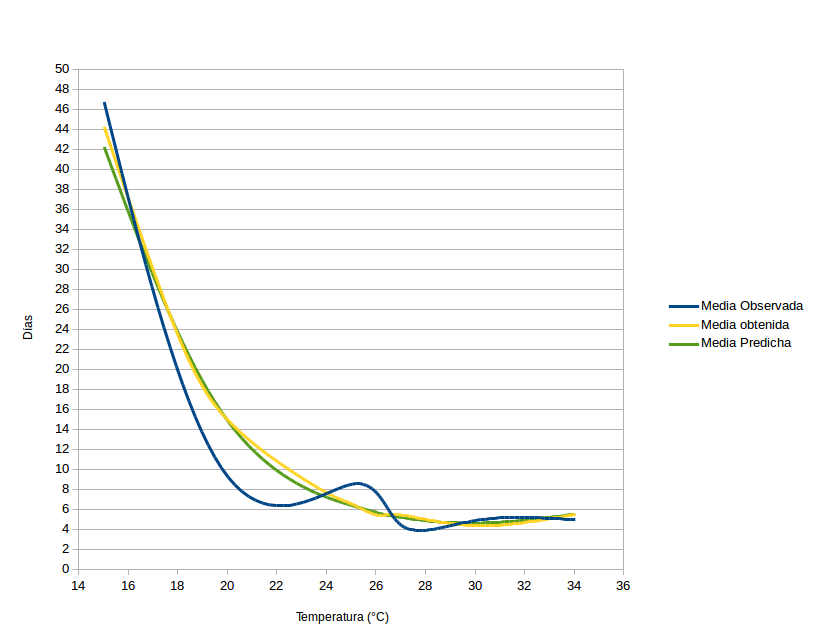
\includegraphics[width=1\textwidth]{capitulo-6/graphics/desarrollo-larva-rueda.png}
    \caption{\label{fig:desarrollo-larva-rueda1990}
    Comparativa entre ,la media obtenida, la media predicha y las media observada por \cite{
    rueda1990temperature} en distintas pobalciones a 6 temperaturas contantes (15-34 \textcelsius)
    para las tasas de desarrollo de las larvas del Aedes Aegypti.}
\end{figure}

%Comparación con los datos de BASERRA

En \cite{BESERRA2006}, se presentan los requerimientos térmicos para el desarrollo del aedes
aegypti en condiciones naturales, para 5 cepas de Aedes Aegyti, provenientes de diferentes
poblaciones, a 5 temperaturas constantes (18-34\textcelsius). En la
\tabref{tab:desarrollo-larva-baserra2006-test} se presentan los resultados obtenidos a cinco
temperaturas constantes(15-34 \textcelsius) en comparación a las tasas de desarrollo obtenidas en
\cite{BESERRA2006} para las larvas del Aedes Aegypti.

\begin{table}[H]
    \begin{minipage}{\textwidth}
    \centering
        \caption{\label{tab:desarrollo-larva-baserra2006-test} Análisis de la tasa de desarrollo de
        las larvas del Aedes Aegypti a cinco temperaturas constantes (15-34 \textcelsius).}
        \begin{tabular}{p{5cm} c c c c c c }
            \hline\\
            Población    &18 \textcelsius & 22 \textcelsius & 26 \textcelsius & 30 \textcelsius
            & 34 \textcelsius & Media General\\
            \hline
            \hline \\
            Boqueirão$^{a}$        & 19,6  & 13,4  & 8,7  & 6,4  & 6,9 & 11\\
            B, dos Santos$^{a}$    & 18,9  & 13,4  & 10,2 & 7,9  & 7,5 & 11,6\\
            C, Grande$^{a}$        & 18,3  & 11,1  & 6,6  & 5,8  & 6   & 9,6\\
            Itaporanga$^{a}$       & 21    & 12,3  & 7,3  & 5,9  & 9,7 & 11,2\\
            Remígio$^{a}$          & 18,9  & 15,8  & 8,4  & 5,4  & 6   & 10,9\\
            Media obtenida$^{b}$   & 23,37 & 10,85 & 5,51 & 4,47 & 5,6 & 9,96\\
        \end{tabular}
        \footnotetext[1]{Los valores presentados para estas poblaciones fueron tomados de
         \cite{BESERRA2006}.}
        \footnotetext[2]{Resultados obtenidos mediante el proceso evolutivo.}
    \end{minipage}
\end{table}


En la \figref{fig:desarrollo-larva-baserra2006}, se puede observar una compartiva con los
valores observados en \cite{BESERRA2006}, la media predicha y la media obtenida. En general se
obtuvo un desarrollo de $9,96$ días para 5 temperaturas contantes (18, 22, 26, 30, 34
\textcelsius), con una diferencia de $1,04$, $1,64$, $-0,36$, $1,24$ y $0,94$ días con la media
general de los valores observados en \cite{BESERRA2006} para las poblaciones de Boqueirão, B. dos
Santos, C. Grande, Itaporanga y Remígio respectivamente. En relación a la media predicha, que fue
obtenida mediante el modelo de \cite{sharpe1977reaction}, se obtuvo una diferencia de $-0,22$ días
con la media obtenida.

\begin{figure}[H]
\begin{minipage}{\textwidth}
    \begin{tabular}{c c }
        \initbox
        \num\putindeepbox[7pt]{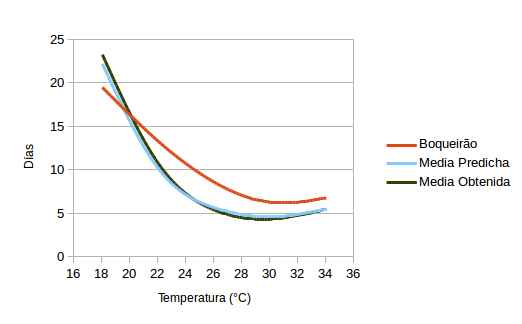
\includegraphics[width=0.4\textwidth]{capitulo-6/graphics/desarrollo-larva-1.png}} &
        \num\putindeepbox[7pt]{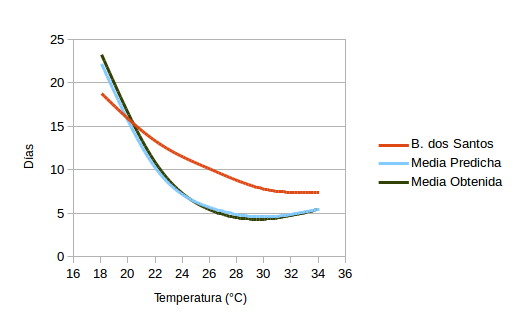
\includegraphics[width=0.4\textwidth]{capitulo-6/graphics/desarrollo-larva-2.png}} \\

        \num\putindeepbox[7pt]{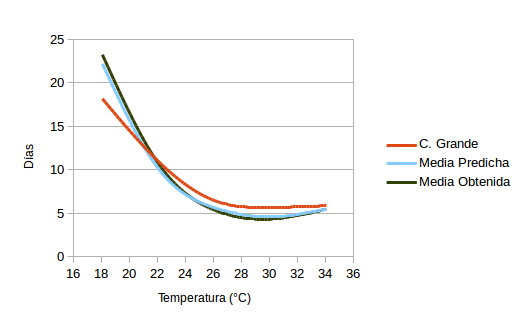
\includegraphics[width=0.4\textwidth]{capitulo-6/graphics/desarrollo-larva-3.png}} &
        \num\putindeepbox[7pt]{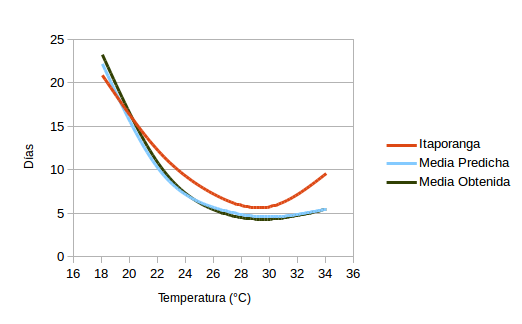
\includegraphics[width=0.4\textwidth]{capitulo-6/graphics/desarrollo-larva-4.png}} \\

        \num\putindeepbox[7pt]{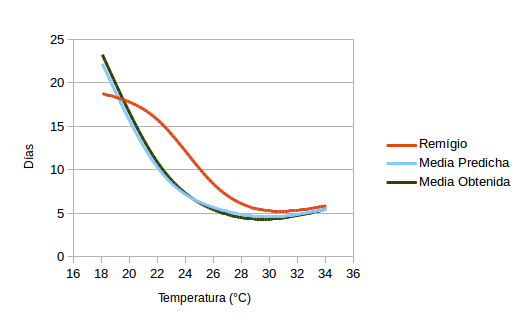
\includegraphics[width=0.4\textwidth]{capitulo-6/graphics/desarrollo-larva-5.png}} &
        \num\putindeepbox[7pt]{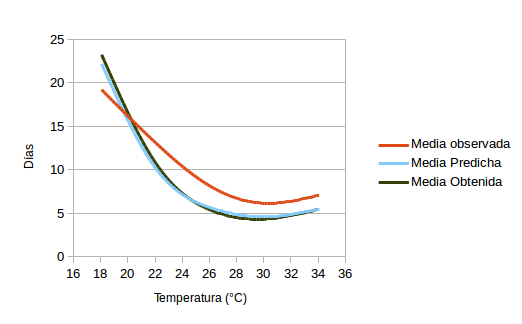
\includegraphics[width=0.4\textwidth]{capitulo-6/graphics/desarrollo-larva-6.png}} \\
    \end{tabular}

    \caption{\label{fig:desarrollo-larva-baserra2006}
    Comparativa entre ,la media obtenida, la media predicha y las medias observadas por \cite{
    BESERRA2006} en distintas pobalciones a 4 temperaturas contantes (18-34 \textcelsius) para
    las tasas de desarrollo de las larvas del Aedes Aegypti.}

    \footnotetext[1]{Tasa de desarrollo de Boqueirão en comparación con la media predicha y obtenida.}
    \footnotetext[2]{Tasa de desarrollo de B. dos Santos en comparación con la media predicha y obtenida.}
    \footnotetext[3]{Tasa de desarrollo de C. Grande en comparación con la media predicha y obtenida.}
    \footnotetext[4]{Tasa de desarrollo de Itaporanga en comparación con la media predicha y obtenida.}
    \footnotetext[5]{Tasa de desarrollo de Remígio en comparación con la media predicha y obtenida.}
    \footnotetext[6]{Media observada en los poblados de Boqueirão, B. dos Santos, C. Grande, Itaporanga, Remígio en comparación con la media predicha y obtenida.}

\end{minipage}
\end{figure}
